\section{Low-level operators and computational cost}
\label{sec:operators}

\subsection{An operator boundary that preserves the discretization}

The nonlinear stage begins after radial reconstruction has produced the angular half-spectra of the physical fields. It ends before radial projection or construction of the finite-difference right-hand side. This boundary is essential: a replacement kernel is required to compute the same dealiased products from the same reconstructed coefficients. Reducing the number of time samples, changing the quadrature, or replacing a weak flux form by a different discrete convection form would alter the method and requires a separate accuracy study. None of those changes is implicit in the fusion described here.

Let \(q\) denote the number of radial rows for this stage, \(N\) the angular transform length, and \(H_N=\lfloor N/2\rfloor+1\) the half-spectrum width. The layout is field-major, with address \(((c q+i)H_N+k)\) for field \(c\), row \(i\), and nonnegative mode \(k\). Each element is a complex FP64 pair. The Galerkin path reads three planes for \(u_r,u_\theta,\omega\) and returns two planes for \(u_r\omega,u_\theta\omega\). The FD path reads four planes and returns one for the sum of two derivative products; its radial metric factors are supplied by the existing reconstruction and right-hand-side conventions. The FD independent mean forcing is supplied separately and retains the original ascending modal sum. Both variants copy the previous raw flux into the prescribed SBDF2 history buffer before overwriting the current buffer.

The reference implementation makes one batched inverse cuFFT call, a product-kernel call, and one batched forward cuFFT call. A batch contains many field--row transforms. Counting three API-level operations is therefore different from counting three individual transforms, and a cuFFT call may itself launch several device kernels\cite{r11}. Galerkin requires three real inverse and two real forward transforms per row; FD requires four inverse and one forward. Both have five logical field transforms. The optimization preserves this logical work and changes its realization.

\begin{figure}[!htbp]
\centering
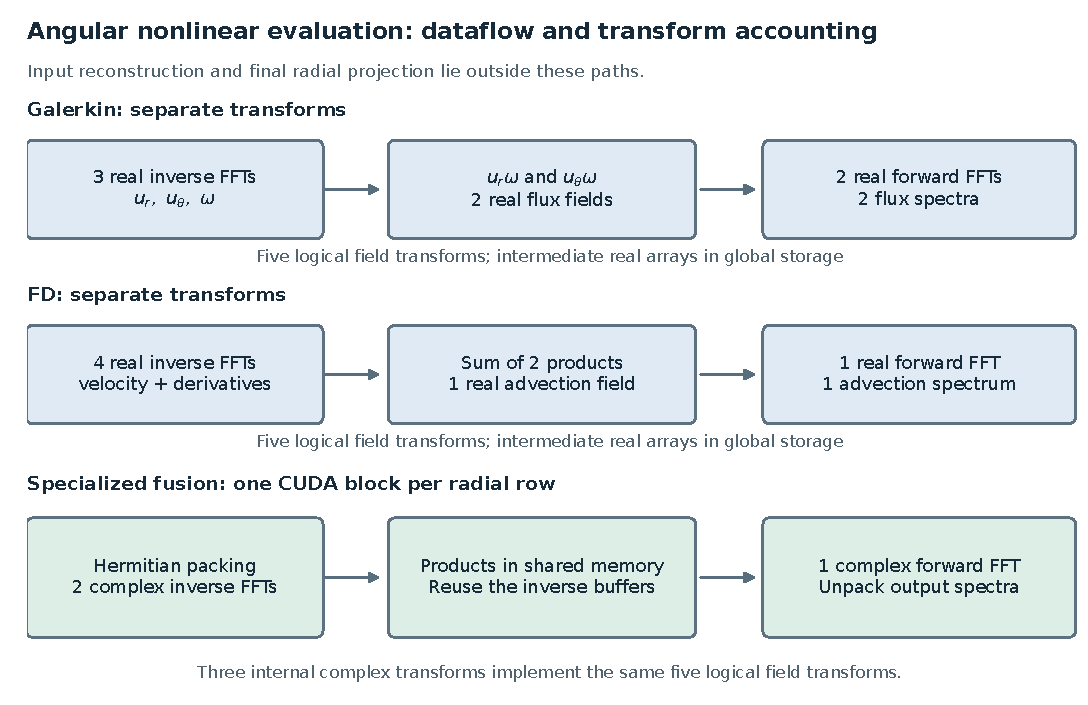
\includegraphics[width=\linewidth]{figures/nonlinear_pipeline.pdf}
\caption{The nonlinear operator boundary. The two discretizations retain their respective field products. Fusion combines the angular transforms, physical products, and packing in shared memory; radial reconstruction and projection lie outside the illustrated replacement. Five logical field transforms remain in both variants.}
\label{fig:operator-pipeline}
\end{figure}

\subsection{Packing identities and normalization}

Define the unnormalized forward and inverse transforms by
\begin{equation}
\label{eq:op-dft}
(\mathcal F_N v)_k=\sum_{j=0}^{N-1}v_j e^{-2\pi\mathrm{i}jk/N},\qquad
(\mathcal B_N A)_j=\sum_{k=0}^{N-1}A_k e^{2\pi\mathrm{i}jk/N}.
\end{equation}
Thus \(\mathcal B_N\mathcal F_N=N I\). The CUDA replacement follows the cuFFT convention\cite{r11}; it does not insert an additional \(1/N\). In the solver, the corresponding normalization already belongs to the following projection or FD right-hand side. Applying it in both locations would change the nonlinear equation, even if a standalone round-trip transform appeared correct.

For two separately Hermitian spectra \(A,B\), linearity gives
\begin{equation}
\label{eq:op-inverse-pack}
\mathcal B_N(A+\mathrm{i}B)=a+\mathrm{i}b,
\qquad a=\mathcal B_N A\in\mathbb R^N,\quad b=\mathcal B_N B\in\mathbb R^N.
\end{equation}
The negative modes must be reconstructed as \(\overline{A_k}+\mathrm{i}\overline{B_k}\). Conjugating the packed positive mode as a whole instead produces \(\overline{A_k}-\mathrm{i}\overline{B_k}\) and is incorrect. The packed sequence is generally not Hermitian. At zero frequency, and at Nyquist frequency for even \(N\), each original real-field coefficient has zero imaginary part.

After forming two real products \(g,h\), let \(Z=\mathcal F_N(g+\mathrm{i}h)\). Their separate spectra follow from
\begin{equation}
\label{eq:op-forward-pack}
G_k=\frac{Z_k+\overline{Z_{-k}}}{2},\qquad
H_k=\frac{Z_k-\overline{Z_{-k}}}{2\mathrm{i}}.
\end{equation}
The Galerkin implementation uses one packed inverse for the two velocities, one inverse for vorticity, and one packed forward for the two fluxes. The FD implementation packs the two velocities and the two derivatives separately, forms their dot product, and performs one forward transform. Consequently both use three internal complex transforms. This accounting is an implementation identity, not evidence of a factor \(5/3\) speedup: real cuFFT transforms exploit Hermitian redundancy already, and the packing, permutation, synchronization, and instruction costs must also be paid.

For a retained band \(|k|\le K\), quadratic products have support at most \(2K\). An aliased contribution into a retained mode would require \(|k+\ell N|\le2K\) for some nonzero integer \(\ell\). Since \(|k+\ell N|\ge N-K\), the strict condition \(N>3K\) excludes such a contribution. This is the standard retained-band dealiasing argument\cite{r13}. It does not imply that modes above \(K\) vanish in the product, nor does it remove radial quadrature error. The replacement preserves the original padded angular grid and truncation.

\subsection{Block mapping, synchronization, and memory traffic}

One 128-thread block handles one radial row. Two shared arrays of \(N\) complex doubles hold the packed inverse inputs and physical fields. The specialized lengths and factorizations are \(200=2^3 5^2\), \(225=3^2 5^2\), and \(243=3^5\). Their shared storage is respectively 6400, 7200, and 7776 bytes per block. These are the supported kernel instantiations; the code is not a general arbitrary-length FFT service.

Let the ordered radices be \(r_0,\ldots,r_{s-1}\), and express an input position using mixed-radix digits \(d_j\). The load permutation is
\begin{equation}
\label{eq:op-permutation}
p(i)=\sum_{j=0}^{s-1}d_j\frac{N}{\prod_{\ell=0}^{j}r_\ell},\qquad
i=\sum_{j=0}^{s-1}d_j\prod_{\ell=0}^{j-1}r_\ell.
\end{equation}
At a stage with previous-radix product \(m\) and current radix \(r\), disjoint butterflies combine positions separated by \(m\), after the appropriate twiddle multiplication. Each thread visits butterflies in strides of 128. A block barrier separates consecutive stages. This is a classical mixed-radix FFT construction; the project contribution is its specialized mapping within this operator boundary, not a new FFT factorization.

The complete sequence is: load the two packed inverse planes in permuted order; execute the inverse stages; retain each thread's one or two physical products in registers; synchronize all reads; overwrite the first shared plane with the permuted products; execute the forward stages; unpack and store the output half-spectra. The register retention and barrier before overwrite are necessary because another thread may still need the old inverse output. Omitting that barrier introduces a read/write race despite using a single block. Including initial-load and overwrite barriers, the number is \(2s+3\), or 13, 11, and 13 for the supported lengths.

The separate implementation materializes inverse physical arrays and forward product arrays in global memory. Counting writes and reads of these named arrays gives a nominal source-level reduction of \(80Nq\) bytes per nonlinear evaluation in either variant. For Galerkin, the count is \((3+3+2+2)Nq\) doubles; for FD it is \((4+4+1+1)Nq\) doubles. This is an access model for the named real arrays, not a bound on total eliminated device traffic. It excludes cache reuse, compiler behavior, library workspaces, and traffic still required for spectral input, flux output, and flux history. It must not be reported as measured DRAM traffic or converted directly into a bandwidth speedup.

Fusion also increases shared-memory use, register lifetimes, and per-block work. The specialized row count may expose too few blocks to saturate a GPU, while consumer hardware may have limited FP64 throughput. Therefore reduced temporary storage does not by itself establish whether the resulting kernel is bandwidth-bound, instruction-bound, or latency-bound. A roofline or occupancy conclusion would require hardware counters and controlled measurements not collected in this study.

\subsection{Floating-point limits and a guarded standalone extraction}

Equations~\eqref{eq:op-inverse-pack}--\eqref{eq:op-forward-pack} hold in exact arithmetic. In floating-point arithmetic, a packed channel of characteristic magnitude \(A\) can introduce an absolute perturbation on the scale of \(\epsilon A\) into a second channel of magnitude \(B\). The corresponding relative scale is \(\epsilon A/B\), before considering transform constants or cancellation. This is an explanatory scale estimate, not an error bound for this kernel. It explains why a combined-vector norm can hide a poor relative error in a weak output. Near-cancelling product sums require an additional absolute error scaled by the magnitudes of the uncancelled terms.

The revision extracts the original CUDA file and its existing CPU model without modifying their bytes, and adds a solver-independent harness with new NumPy and direct-convolution oracles. The input contract checks supported lengths, FP64 contiguous layouts, real endpoints, zero padding, finite data, and valid retained bandwidth. As a new engineering guard, the adapter rejects a pair of nonzero packed input spectra if the smaller per-row maximum magnitude is less than \(10^{-8}\) times the larger. The threshold is a conservative dispatch policy, not a sufficient condition for a relative-error theorem. Exactly zero channels instead require an absolute-error check. A production integration would need a verified unpacked fallback and a low-cost way to obtain the relevant scales; neither is claimed here. The frozen NS kernels and their qualification records are unchanged.

The harness was run on the local GPU for 36 fixed-state cases: three lengths, two variants, and six fixture classes per variant. The sixth class is a zero velocity channel for Galerkin and additive cancellation for FD, giving seven distinct labels across the two variants. It uses both an independent NumPy FFT oracle and an FFT-free retained-band convolution oracle; it also checks flux history and FD mean-buffer parity. For each output channel, the relative metric is the infinity-norm ratio \(\max_{i,k}|Y_{ik}-Y^{\rm ref}_{ik}|/\max_{i,k}|Y^{\rm ref}_{ik}|\), over all radial rows and half-spectrum modes, not a pointwise relative error. Ordinary cases attained a maximum channel-relative error of \(1.18\times10^{-15}\). The absolute diagnostic uses one common scale across channels: the maximum, over output channels and rows, of \(N\) times the sum of the products of the separate physical-field maximum magnitudes in each flux expression. Across all fixtures, the largest absolute error divided by this uncancelled scale was \(3.84\times10^{-16}\). Because this common scale can hide errors in a weak channel, it must be read together with the per-channel relative metrics. Deliberately reducing one velocity channel by \(10^{-10}\), after confirming rejection by the guard and explicitly overriding it for diagnosis, produced a maximum channel-relative error of \(4.98\times10^{-6}\). These rounded-up figures describe new synthetic verification, distinct from the earlier archived operator measurements. No new timing or NS trajectory was collected for this extraction. It is distributed as a local contribution candidate in the supplementary source package.

\subsection{Observation reduction and CPU kernels}

The probe operator evaluates six weighted sums, \(p_j=w_j^\top x+\ell_j(t)\). The old implementation assigned each sum to one thread. The replacement assigns a complete warp to each probe: lane \(\ell\) accumulates indices \(\ell+32m\), then five shuffle reductions combine lane values\cite{r18}. A block of 192 threads therefore covers all six probes. The arithmetic work remains linear in the frame length; the per-probe serial depth is reduced from roughly \(L\) to \(\lceil L/32\rceil+5\), ignoring instruction and memory costs. Snapshot copies, selected state pointers, and synchronization before advancing the state are preserved. Reordering additions changes rounding, so bitwise state preservation and numerical probe agreement are separate assertions. This common observation improvement is applied to both Galerkin and FD comparisons.

There are also project-local C implementations below the Python driver. The Galerkin contraction kernel places the angular mode in the contiguous inner loop and combines the same precontracted mass and flux projections. The buffered FD kernel applies already assembled narrow radial stencils, reuses working arrays, and forms physical products in place. A separate band solver applies cached real LAPACK factor data to interleaved complex right-hand sides. The FD build specifies optimization and AVX2 support while disabling fused multiply-add contraction; that compiler option alone does not certify SIMD utilization or a speedup. SciPy still provides selected FFTs or factorization services in these CPU variants. The project does not replace their algorithms or patch their source.

These implementations demonstrate genuine low-level changes, but their existence is not an isolated end-to-end timing result. Likewise, replacing the Python orchestration language with Rust would not directly reduce the device FFT work, retained rank, or compiled-kernel initialization. A language migration would be justified only by a measured host bottleneck or a reusable interface requirement. The current attribution distinguishes loop/layout changes from module import, compilation caching, and CUDA graph scheduling.

\subsection{Costs, amortization, and upstream scope}

For attribution, write the total cost as
\begin{equation}
\label{eq:cost}
\begin{aligned}
T_{\rm total}={}&T_{\rm start}+T_{\rm prepare}+N_{\rm nl}C_{\rm nl}\\
&+N_{\rm step}C_{\rm lin}+N_{\rm obs}C_{\rm obs}+T_{\rm finish}.
\end{aligned}
\end{equation}
The costs denote phase-weighted effective quantities, not an assertion that every step costs the same. Here \(C_{\rm lin}\) excludes the nonlinear and observation terms already counted. Time-grid optimization changes \(N_{\rm nl}\) and \(N_{\rm step}\); fusion changes \(C_{\rm nl}\); warp reduction changes \(C_{\rm obs}\); and preparation reuse or caching changes other terms. Their savings cannot be added across unrelated measurements or counted twice.

If a fraction \(f\) of an otherwise fixed execution is accelerated by a local factor \(s\), the corresponding ideal bound is \([1-f+f/s]^{-1}\). An additional initialization cost makes the gain smaller. More explicitly, let \(S_b,S_f\) be setup costs and \(B_b,B_f\) the costs of one otherwise matched repeated workload. Under genuine reuse of setup, the fused path wins after \(m\) repetitions only if
\begin{equation}
\label{eq:op-amortization}
m(B_b-B_f)>S_f-S_b.
\end{equation}
If each new process rebuilds or reloads the relevant state, setup is not a once-only term and this amortization model must be changed. The fixed-state event measurements and short-trajectory results in the next section illustrate precisely why the distinction matters. An explicit PTX cache also does not eliminate all driver JIT, loading, context, planning, or process-start costs.

The complete-solve clock includes construction, compilation or loading, transfers, FFT preparation, graph capture, advancement, observation, synchronization, download, and resource release. The new-process clock additionally includes interpreter startup, imports, and the prescribed supervision overhead. Neither clock can be replaced by isolated kernel events. Numerical qualification may use concurrent independent jobs, but latency comparison requires serialized GPU use and monitored external activity. Aggregate CPU utilization is not an accuracy-constrained performance metric.

Finally, the source audit found project-local application kernels and library calls, not an identified modification to borrowed cuFFT, cuFFTDx, SciPy, or LAPACK source. NVIDIA already provides FFT fusion and convolution examples, including comparisons with a cuFFT pipeline and optional LTO callbacks\cite{r17}. The plausible upstream contribution is therefore a new multifield FP64 inverse-transform--cross-product--forward-transform example, not a claim to have invented FFT fusion or repaired cuFFT. A useful proposal still requires an equivalently fused cuFFTDx implementation, a batched cuFFT baseline, matched precision and padding, first-use and repeated-use costs, and a clean build outside this machine. The local extraction has not satisfied those performance and portability requirements, has not established a new license grant or contribution certification, and has not been submitted as a PR\cite{r19}.

\subsection{Maintenance of the early steady-solver interface}
The dynamic replacement cited by the reviewer belongs to an early steady-cavity
control: its wrapper temporarily replaced
\path{rfm_v2_solver.trial_basis}, outside the final annular solver path.
We preserve the archived source hashes and provide a separate maintained package
with an explicit, solve-local basis factory. Omitting this argument preserves the
default behavior; the mapped-Legendre wrapper no longer changes module globals.
All seven CPU tests pass. Eight small configurations agree with the archived
functions in coefficients, Stokes matrices, and velocity, vorticity and other fields
at 25 independent points, using relative and absolute tolerances of $10^{-12}$.
Additional tests force concurrent factory overlap and check default calls after
factory and assembly exceptions. These establish interface compatibility and
state isolation for this change; they provide no new annular accuracy certificate,
GPU speed result, or thread-safety guarantee for arbitrary user-supplied factories.

